\documentclass{sigchi}

% Use this command to override the default ACM copyright statement
% (e.g. for preprints).  Consult the conference website for the
% camera-ready copyright statement.


%% EXAMPLE BEGIN -- HOW TO OVERRIDE THE DEFAULT COPYRIGHT STRIP -- (July 22, 2013 - Paul Baumann)
% \toappear{Permission to make digital or hard copies of all or part of this work for personal or classroom use is      granted without fee provided that copies are not made or distributed for profit or commercial advantage and that copies bear this notice and the full citation on the first page. Copyrights for components of this work owned by others than ACM must be honored. Abstracting with credit is permitted. To copy otherwise, or republish, to post on servers or to redistribute to lists, requires prior specific permission and/or a fee. Request permissions from permissions@acm.org. \\
% {\emph{CHI'14}}, April 26--May 1, 2014, Toronto, Canada. \\
% Copyright \copyright~2014 ACM ISBN/14/04...\$15.00. \\
% DOI string from ACM form confirmation}
%% EXAMPLE END -- HOW TO OVERRIDE THE DEFAULT COPYRIGHT STRIP -- (July 22, 2013 - Paul Baumann)


% Arabic page numbers for submission.  Remove this line to eliminate
% page numbers for the camera ready copy 

%\pagenumbering{arabic}

% Load basic packages
\usepackage{balance}  % to better equalize the last page
\usepackage{graphics} % for EPS, load graphicx instead 
%\usepackage[T1]{fontenc}
\usepackage{txfonts}
\usepackage{times}    % comment if you want LaTeX's default font
\usepackage[pdftex]{hyperref}
% \usepackage{url}      % llt: nicely formatted URLs
\usepackage{color}
\usepackage{textcomp}
\usepackage{booktabs}
\usepackage{ccicons}
\usepackage{todonotes}

\usepackage{paralist}

% llt: Define a global style for URLs, rather that the default one
\makeatletter
\def\url@leostyle{%
  \@ifundefined{selectfont}{\def\UrlFont{\sf}}{\def\UrlFont{\small\bf\ttfamily}}}
\makeatother
\urlstyle{leo}

% To make various LaTeX processors do the right thing with page size.
\def\pprw{8.5in}
\def\pprh{11in}
\special{papersize=\pprw,\pprh}
\setlength{\paperwidth}{\pprw}
\setlength{\paperheight}{\pprh}
\setlength{\pdfpagewidth}{\pprw}
\setlength{\pdfpageheight}{\pprh}

% Make sure hyperref comes last of your loaded packages, to give it a
% fighting chance of not being over-written, since its job is to
% redefine many LaTeX commands.
\definecolor{linkColor}{RGB}{6,125,233}
\hypersetup{%
  pdftitle={Edvertisements: Adding Microlearning to Social News Feeds and Websites},
  pdfauthor={LaTeX},
  pdfkeywords={SIGCHI, proceedings, archival format},
  bookmarksnumbered,
  pdfstartview={FitH},
  colorlinks,
  citecolor=black,
  filecolor=black,
  linkcolor=black,
  urlcolor=linkColor,
  breaklinks=true,
}

% create a shortcut to typeset table headings
% \newcommand\tabhead[1]{\small\textbf{#1}}

% End of preamble. Here it comes the document.
\begin{document}

\title{Edvertisements: Adding Microlearning to \\ Social News Feeds and Websites}

\numberofauthors{3}
\author{%
  \alignauthor{Anonymized for review\\
    \affaddr{Affiliation}\\
    \affaddr{City, Country}\\
    \email{e-mail address}}\\
}

\maketitle

%\begin{textblock}{5}(3.6,7.7)
%\begin{figure}
%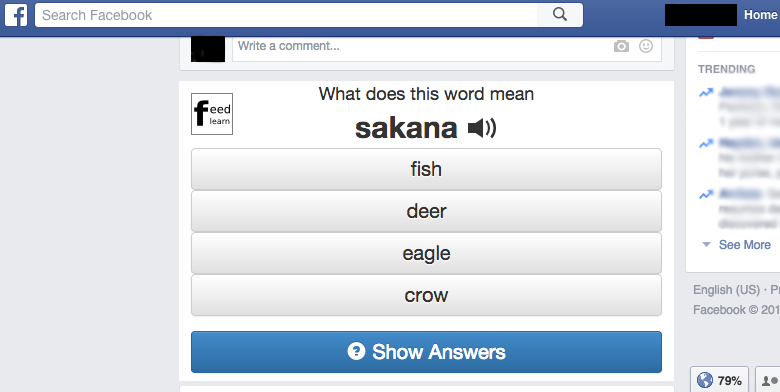
\includegraphics[width=\columnwidth]{feedlearn-screenshot.png}
%\caption{FeedLearn showing an interactive vocabulary quiz inside a user's Facebook news feed}
%\label{fig:feedlearn}
%\end{figure}
%\end{textblock}

\begin{figure}
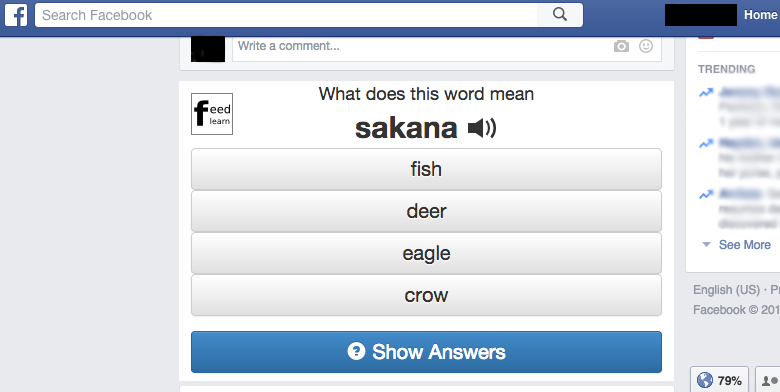
\includegraphics[width=\columnwidth]{feedlearn-screenshot.png}
\caption{Our extension can show interactive microlearning tasks (Edvertisements) in users' Facebook news feeds.}
\label{fig:feedlearn}
\end{figure}

\begin{figure}
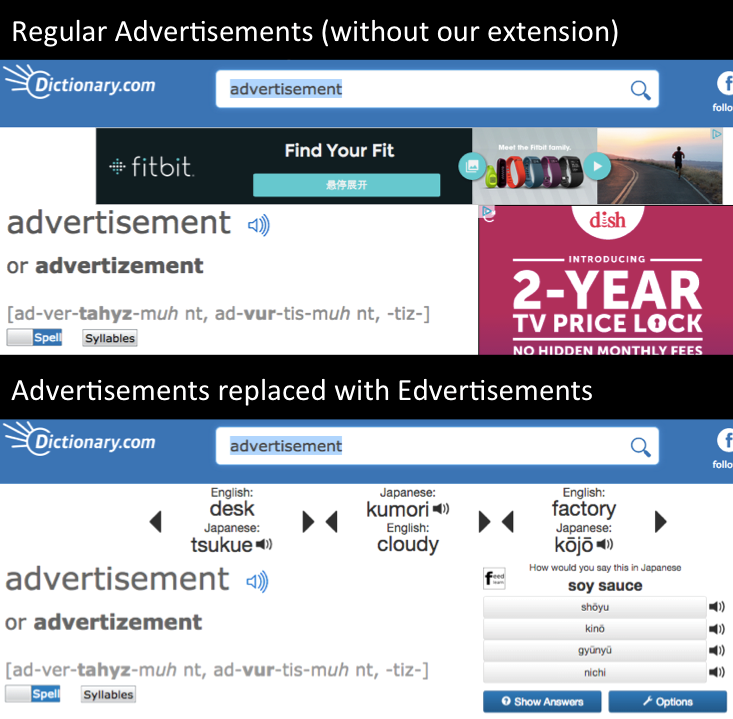
\includegraphics[width=\columnwidth]{edvertisements-screenshot4.png}
\caption{Our extension can replace advertisements with interactive microlearning tasks (Edvertisements) on arbitrary websites.}
\label{fig:edvertisements}
\end{figure}

\begin{abstract}
Many long-term goals, such as learning a language, require people to regularly practice every day to achieve mastery. At the same time, people regularly surf the web and read social news feeds in their spare time. We have built a browser extension that teaches vocabulary to users in the context of Facebook feeds and arbitrary websites, by showing users interactive quizzes they can answer without leaving the website. On Facebook, the quizzes are shown as part of the news feed, while on other sites, the quizzes appear where advertisements normally would. In our user study, we examined the effectiveness of inserting microlearning tasks into social news feeds.
We compared vocabulary learning rates when we inserted interactive quizzes into feeds, versus inserting links that lead them to a website where they could do the quizzes. Our results suggest that users engage with and learn from our embedded quizzes, and engagement increases when the quizzes can be done directly within their feeds.
% We compared vocabulary learning rates when interactive quizzes were inserted directly into feeds, versus inserting links that lead them to quizzes. Our results suggest that users engage with and learn from our embedded quizzes, and engagement increases when the quizzes can be done directly within their feeds.
% Many long-term goals, such as learning a language, require people to spend a small amount of time each day to achieve them. At the same time, people regularly surf the web and read social news feeds in their spare time. We have built a browser extension that teaches vocabulary in the context of Facebook feeds and arbitrary websites, by showing users interactive quizzes they can answer without leaving the website. On Facebook, the quizzes are shown as part of the news feed, while on other sites, the quizzes are shown where advertisements would normally appear. In our user study, we looked at the effectiveness of inserting microlearning tasks into social news feeds. We compared vocabulary learning rates when interactive quizzes were inserted directly into feeds, versus inserting links that lead them to quizzes. Our results suggest that users engage with and learn from our inserted quizzes, and engagement is higher when they can be done directly inside their feeds.
%Many long-term goals, such as learning a language, require people to spend a small amount of time each day to achieve them. At the same time, people regularly surf the web and read social news feeds in their spare time. We have built a browser extension that teaches vocabulary in the context of Facebook feeds and arbitrary websites, by showing users interactive quizzes they can answer without leaving the website. On Facebook, the quizzes are shown as part of the news feed, while on other sites, the quizzes are shown where advertisements would normally appear. In our preliminary user study, we looked at the effectiveness of inserting microlearning tasks into social news feeds. We compared Japanese vocabulary learning rates when interactive quizzes were inserted directly into feeds, versus inserting links that lead them to quizzes. Our results suggest that users engage with and learn vocabulary from our inserted quizzes, and they engage more with microlearning tasks when they can be done directly inside their feeds.
% In our preliminary user study, we find that over the course of a week, we are able to teach students an average of 13 new vocabulary words by injecting microlearning tasks into their Facebook feeds. This is more than the 4 vocabulary words learned if we insert links leading them to visit an external site to study, as is done by current Facebook apps.
% Unlike apps like Duolingo posting accomplishments in users' feeds, FeedLearn gives friends a simple call to action and allows them to participate in their friends' learning processes.
%In our first study, we find that over the course of 2 weeks, we are able to teach students N new vocabulary words by injecting microlearning tasks into their Facebook feeds. This is X\% more than a control condition where we ask them to visit a separate website and ask them to study the words on their own time, and Y\% more than a control condition where we show friends' achievements via feed updates. In our second study, we find that giving friends the ability to participate in the social learning process, by suggesting words for their friends to learn, leads to increased engagement. They learn more words in a condition where the words learned are suggested to the group by their friends, which is X\% more than when they select words to choose by themselves, and Y\% more than when the suggestions are automatic.
\end{abstract}

\keywords{microlearning; social feeds; facebook; advertisements; language learning}

\category{H.5.2.}{User Interfaces}{Graphical user interfaces (GUI)}{}{}
% \category{H.5.m.}{Information Interfaces and Presentation (e.g. HCI)}{Miscellaneous}

%\newpage

\section{Introduction}

% we should first talk about the problem: the difficulty and importance of getting people to regularly do learning tasks. darren's papers had some citations
% People want to learn new languages, but the commitment is too much effort for them, especially when regular practice is a prerequisite.

Many people have long-term learning goals, such as wanting to learn a new language. However, they often fail to achieve these goals, citing the lack of time to study as a major reason \cite{micromandarin, kam2007localized, oxford1994language}.
Nevertheless, people do have spare time, as shown by their recreational web browsing and social network usage. % regularly visit social networking sites and browse the web.
% Americans spend 27 hours per month web browsing \cite{nielsen2014},  %-- they spend large amounts of time surfing the web and reading social news feeds on sites like Facebook.
American adults spend an average of 27 hours per month surfing the web \cite{nielsen2014}.
71\% of American adults use Facebook, and 63\% of these visit Facebook daily \cite{socialmediaupdate}. 90\% of American college students use Facebook, spending on average of 30 minutes on Facebook each day \cite{collegefacebook2}. % Hence, we aim to help people study during their recreational web usage. % Among American college students, 90\% use Facebook \cite{collegefacebook2}, spending an average of 30 minutes per day on it \cite{collegefacebook}. % Social news feeds are widely used - over half of college students who use Facebook report reading their Facebook news feeds 5-7 days per week \cite{collegefacebook}. % Social news feeds and % Clearly, Facebook news feeds present an opportunity for influencing the behavior of users.

%American adults spend an average of 27 hours per month browsing the web \cite{nielsen2014}.
%71\% of American adults with an internet connection use Facebook. Of these, 63\% visit Facebook at least once a day, and 40\% visit it multiple times per day \cite{socialmediaupdate}. Among American college students, 90\% use Facebook \cite{collegefacebook2}, spending an average of 30 minutes per day on it \cite{collegefacebook}. Social news feeds are widely used - over half of college students who use Facebook report reading their Facebook news feeds 5-7 days per week \cite{collegefacebook}. % Social news feeds and % Clearly, Facebook news feeds present an opportunity for influencing the behavior of users.

% Some notes about microlearning and learning would be useful here: daily practice matters, burden in opening separate apps and context switch, etc. 

In this paper, we present \textit{Edvertisements}, which help users learn during their spare time by showing them interactive microlearning tasks as they surf the web and read their Facebook feeds. We implemented a Chrome extension which shows Edvertisements in two ways:

% In this paper, we present \textit{Edvertisements}, which shows interactive microlearning tasks to users as they browse the web and read their Facebook feeds. We implemented a Chrome extension which shows Edvertisements in two ways:

% In this paper, we present Edvertisements, interactive microlearning tasks which we show to users as they browse the web and read their Facebook feeds. We implemented a Chrome extension which shows Edvertisements in two ways:

\begin{compactitem}
\item On Facebook, the extension embeds Edvertisements directly into the feed alongside regular posts (see \autoref{fig:feedlearn}).
%\item On Facebook, Edvertisements are inserted into the feed, alongside regular feed items.
\item On other sites, the extension replaces web advertisements with Edvertisements (see \autoref{fig:edvertisements}). % shows Edvertisements in areas where advertisements would normally appear. % Edvertisements appear in areas where advertisements would normally appear.
% \item On other sites, Edvertisements are shown in locations where advertisements would normally appear.
\end{compactitem}

\pagebreak

Our research questions are:

\begin{compactitem}
\item Do users engage with and learn from Edvertisements that we insert into their Facebook feeds?
\item Do users engage more with Edvertisements if they can do the microlearning tasks without leaving their Facebook feeds (compared to external links)?
% \item Does having Edvertisements where users can do the microlearning tasks without leaving their Facebook feeds result in higher learning outcomes?
% \item Does the regularity and frequency with which users visit Facebook make it suitable for microlearning?
%\item Are people more likely to learn if they are shown small, easily actionable learning tasks in the social feed. %, instead of messages emphasizing friends' overall achievements?
%\item  Are people more likely to do flashcards that their friends suggested for them to do, as opposed to flashcards they selected themselves, or flashcards suggested by the system?
%\item  Are people more likely to do flashcards that they suggested to their friends for them to do, as opposed to flashcards they selected only for themselves, or flashcards suggested by the system?
%\item Does the act of suggesting words for friends to learn improve users' engagement with the system, or perceived satisfaction?
%\item Does the selection process result in something useful?
\end{compactitem}

In our user study, we examined engagement and vocabulary acquisition rates after embedding Edvertisements into users' Facebook feeds. We found that users interacted frequently with Edvertisements, improved their post-test results after a week, and engaged more readily with Edvertisements when they did not have to leave their social news feeds.

% In our user study, we examined engagement and vocabulary acquisition when Edvertisments were inserted into users' Facebook feeds, and the effects of being able to do the microlearning tasks in-place. We found that there was high engagement with Edvertisements, users had improved post-test results after a week, and that engagement was higher when Edvertisements could be done in-place.

% In our user study, we looked at engagement and vocabulary acquisition when Edvertisments were inserted into users' Facebook feeds. We also compared the effects of being able to do the microlearning tasks in place, as opposed to having to click a link to go to an external website. We found that there was high engagement with Edvertisements, users had improved post-test results after a week, and that engagement was higher when Edvertisements could be done in-place. % without leaving the feed. % users answered more quizzes when they could do so without leaving the feed, and they learned more new words on average over a week. 

% In our user study, we looked at engagement and vocabulary acquisition when Edvertisments were inserted into users' Facebook feeds. We also compared the effects on engagement and vocabulary acquisition of being able to do the microlearning tasks in place, as opposed to having to click a link to go to an external website. We found that there was high engagement with Edvertisements, users had improved post-test results after a week, and that engagement was higher when the Edvertisements could be done without leaving the feed. % users answered more quizzes when they could do so without leaving the feed, and they learned more new words on average over a week. 

% Our preliminary user study looked at engagement and Japanese vocabulary acquisition rates through FeedLearn's in-feed interactive quizzes, versus inserting links to an external website where they can do quizzes, as is currently done by Facebook applications. We found that users answered more quizzes when they could do so without leaving the feed, and they learned more new words on average over a week. % when they could do the quizzes inside the feeds.

\section{Related Work}

\subsection{Microlearning}

Microlearning is the strategy of studying frequently in short intervals throughout the day \cite{gassler2004integrated}. Several mobile applications use microlearning to teach material such as foreign language vocabulary \cite{microlearning, micromandarin}; however, these require the user to interrupt their routine to open a dedicated app for studying. % . A potential drawback of needing a separate app for microlearning is that it requires the user to develop a habit of interrupting their routine to open an app to study. % Although they may give users reminders when they should practice, these reminders might come at the wrong time, or be ignored.

Some systems try to solve this problem by embedding microlearning into other contexts. There are games in which users complete learning tasks while playing \cite{carriearcade}, video players which teach vocabulary while users watch foreign-language videos \cite{smartsubtitles}, screensavers that display facts while the screen is idle \cite{screensaver}, and chat clients that show vocabulary while the user is chatting \cite{cai2015wait}.

% Compared to the learning contexts used by existing work, we believe that recreational web surfing and Facebook feeds are especially good opportunities for microlearning, because:

Compared to the learning contexts used by existing systems, we believe that web surfing and Facebook feeds are especially potent locations for embedding microlearning, because:

\begin{compactitem}
\item Unlike playing educational games or watching foreign-language videos, visiting Facebook is a daily habit for 45\% of American adults with an internet connection \cite{socialmediaupdate} %, and the majority of college students \cite{collegefacebook}.
% \item Unlike a screensaver which is dismissed once the mouse moves, users can interact with quizzes they see in their Facebook feeds.
%\item Unlike needing to respond to a chat message, there are no interruptions to the user's learning while they are browsing their Facebook feeds.
\item Web surfing and reading Facebook news feeds are recreational activities, so the embedded microlearning tasks will not interrupt users' work.
\item Users are already accustomed to a variety of rich content appearing in their Facebook feeds, such as videos, games, recommendations, and advertisements, so they should not find the added Edvertisements too distracting.
% \item Users are already accustomed to a variety of rich content appearing in their Facebook feeds, such as videos, games, recommendations, and advertisements.
%\item Users are already used to a variety of rich content appearing in their Facebook feeds, such as videos their friends liked, posts from games and apps, recommendations, and advertisements.
\end{compactitem}


%\subsection{Spaced Repetition}

%Spaced repetition is a technique designed to help learners retain information by having them review items at regular intervals \cite{karpicke2011spaced}. A class of applications that exploit this are flashcards, which split information into independent chunks that are scheduled for review based on factors such as mastery and recency of review. There have been a number of algorithms and models designed for optimizing learners' retention of the material via spaced repetition \cite{optimalschedule} \cite{memreflex}.

% \subsection{Using Social News Feeds as a Persuasive Technology}
\subsection{Using Social News Feeds to Trigger Desired Habits}

% should probably cite some of nir eyal and bj fogg's stuff about triggers. ie, to form habits, need motivation, ability, and a trigger -- our in-feed quizzes are the magic trigger that will get people to learn.

Many apps post on users' Facebook feeds to drive engagement. %Facebook feeds.
For example, Duolingo can share users' study progress, and Strava can share users' exercise history.
These posts aim to get users' friends to send them encouraging feedback, and to try the apps themselves.
However, these posts are often viewed as bragging about trivial accomplishments, and receive little attention \cite{socialsharing}. % users are uncomfortable with letting apps post on their feeds, and the posts are viewed as bragging about trivial accomplishments \cite{socialsharing}. % these posts are often ignored, and rarely acted upon \cite{socialsharing}. % However, messages posted by applications receive less attention compared to messages posted by actual users. Viewers may perceive these posts negatively, ignoring them \cite{socialsharing}.

These posts are examples of \textit{triggers}, which are calls to action designed to help users form habits \cite{foggpersuasive}. Facebook app posts require the user to go to a different website to study, as Facebook's API does not allow apps to post interactive content. With Edvertisements, we lower the barrier to action by allowing the user to study without leaving the website.

% Many apps attempt to use Facebook feeds as a persuasive technology, to help users form study habits. For example, apps like Duolingo can broadcast users' study progress on the platform, inviting the user's friends to participate in the activity. However, there are many caveats with such applications auto-posting messages on users' feeds. Messages auto-posted by applications receive less attention from the user's friends, compared to messages posted by actual users. Viewers may perceive these posts negatively, ignoring them \cite{socialsharing}.

\pagebreak

\subsection{Web Advertising and Ad-Blocking}

% Web advertisements are another example of a trigger, though in their case the habit they are attempting to drive is consumption of a product.
Although advertisements are an important revenue source for websites, surveys indicate that 77\% of users rarely ever click on ads, and 69\% express interest in skipping or blocking ads \cite{adblockinggames}.
16\% of US web users use ad blockers, which are browser extensions that prevent web ads from being displayed. Ad blocker usage is growing -- global ad blocking has more than tripled since 2013, and is posed to further grow as ad blockers for mobile devices gain traction \cite{costofadblocking}. % ad blockers emerge.
% 5\% of web users use ad blockers, which are browser extensions that prevent web ads from being displayed \cite{adblockinggoesmainstream}. Ad-blocking is especially common among Chrome and Firefox users -- 30\% of Chrome users and 35\% of Firefox users have installed an ad-blocker \cite{adblockinggoesmainstream}.

% It is also growing quickly -- global ad blocking has more than tripled since 2013, and is posed to further grow as ad blockers for iOS and Android grow commonplace. % ad blockers emerge.

% 16% of web users in the US block ads
% http://downloads.pagefair.com/reports/2015_report-the_cost_of_ad_blocking.pdf

In surveys, users of ad-blockers cite ``distracting animations and sounds'', and ``offensive/inappropriate ad content'' as their top reasons for blocking ads \cite{adblockinggames}. Even users who do not install ad blockers tend to avoid looking at ads, a phenomenon known as ``banner blindness''. In fact, web surfers click on less than 0.5\% of advertisements -- a number which has been declining ever since banner ads were introduced in 1994 \cite{whypeopleavoidadvertising}. Edvertisements repurpose this space for microlearning.

% Although advertisements are an important revenue source for websites, in consumer surveys 77\% report that they hardly ever click on ads, and 69\% express interest in skipping or blocking ads \cite{adblockinggames}. Ad blockers, which are browser extensions that prevent web ads from being displayed, are used by 5\% of all internet users \cite{adblockinggoesmainstream}. Ad-blocking is especially common among Chrome and Firefox users -- 30\% of Chrome users, and 35\% of Firefox users, have installed an ad-blocker \cite{adblockinggoesmainstream}. %with ad-blocking extensions being the most popular extensions in each browser's extension store.

% In surveys, users of ad-blockers cite ``distracting animations and sounds'', and ``offensive/inappropriate ad content'' as their top reasons for blocking ads \cite{adblockinggames}. Although ad-blocking software can be configured to selectively whitelist/blacklist ads for certain websites, most ad-blocker users just retain the default behavior of blocking ads on all websites \cite{adblockinggames}, which may perhaps be due to usability issues in configuring ad-blockers \cite{adblockusability}. %By preventing ads from being shown, ad-blockers pose a threat to the advertising industry, as well as websites which rely on advertising revenue \cite{adblockinggames}. % Some websites such as Hulu have responded to this by detecting the presence of ad-blocking software, and requesting that users disable their ad-blockers, though writers of ad-blocker.

% TODO Today's ad-blockers simply blank out or remove advertisements. With Edvertisements, we aimed to make use of the space to benefit the end user's goals.

% Many apps attempt to use Facebook feeds as a persuasive technology. For example, apps like Duolingo can broadcast users' study progress on the platform, inviting the user's friends to participate in the activity. %A key advantage that social platforms like Facebook provide is that friends can be associated with requests, increasing their potential persuasiveness via social pressures \cite{foggfacebook}.
%Since the emergence of the Facebook app development platform, there have been
%many attempts to use it as a platform for persuasion. For example, apps like NikePlus can broadcast users' running progress, and apps like Duolingo can broadcast users' study progress on the platform. These messages may also invite the user's friends to participate in the activity. A key advantage that social platforms like Facebook provide is that friends can be associated with requests, increasing their potential persuasiveness via social pressures \cite{foggfacebook}.

% However, there are many caveats with such applications auto-posting messages on users' feeds. Messages auto-posted by applications receive little attention from the user's friends, compared to messages that they have posted themselves. Viewers may perceive these posts as either trivial achievements or bragging, ignoring them \cite{socialsharing}. % It is thus suggested that these auto-posted messages be shared only with the subset of the user's friends who are likely to be interested. However, users are unwilling to invest the effort to identify these social circles \cite{socialsharing}.

%\subsection{Study groups on Facebook}

%There are a number of Facebook pages that post daily ``word of the day'' style lessons for learners, such as KoreanClass101. If users subscribe to these pages (by clicking the Like button), they will see periodic reminders to visit an external site to study vocabulary. These services have a number of weaknesses that FeedLearn aims to address:

% There are a number of Facebook pages that post daily ``word of the day'' style lessons for learners, such as KoreanClass101. If users subscribe to these pages (by clicking the Like button), they will see periodic reminders to visit an external site to study vocabulary, as shown in \autoref{fig:learn-korean}. These services have a number of weaknesses that FeedLearn aims to address:

%\marginpar{
%\begin{figure}
%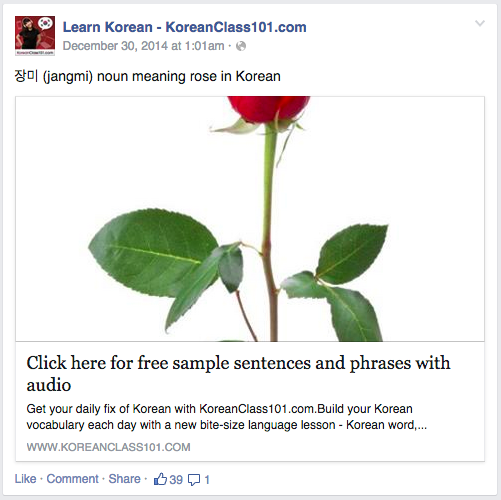
\includegraphics[width=\marginparwidth]{learn-korean-post.png}
%\caption{An example Daily Word post from KoreanClass101, a Facebook service with 70 thousand subscribers.}
%\label{fig:learn-korean}
%\end{figure}
%}

%\begin{compactitem}
%\item Not interactive: users need to visit an external site to do quizzes or see other words.
%\item Not personalized: all 70 thousand subscribers will see the same daily word posted, regardless of whether they already know that word.
%\item No spaced repetition: a new word is posted each day, and older words are never repeated.
%\item Content needs to be manually generated: a group moderator needs to write a new post each day
%\end{compactitem}

% because . These services also generally rely on an external site for 

% ALOE is a system that allows users to learn foreign-language vocabulary while browsing the web, by replacing words in the user's native language with foreign-language vocabulary \cite{augmenting}. This work differs from existing microlearning systems by 

\section{Edvertisements System}

Our system is a Chrome extension that can show users microlearning tasks -- in our case, vocabulary quizzes -- in users' Facebook feeds, and as they are browsing the web. Although we originally implemented the browser extension for Chrome, we have also ported it to Firefox, and our technique can be implemented on any browser that supports extensions (Chrome, Firefox, Edge, Safari, etc). Our system features a variety of microlearning tasks for learning vocabulary in multiple languages, but in this paper we will focus on learning Japanese vocabulary.

% IAB standard container

% Internet Advertising Board

\subsection{Inserting Edvertisements into Facebook Feeds}

Our extension can insert Edvertisements into users' Facebook feeds as rectangular interactive quizzes mimicking the look of a regular feed item, as shown in \autoref{fig:feedlearn}. We chose to insert 1 microlearning task for every 10 normal feed items, to mimic the approximate frequency we observed sponsored content appearing in the feed.

\subsection{Replacing Web Advertisements with Edvertisements}

People spend considerable time on sites other than Facebook, so we also created a general mechanism for presenting microlearning tasks as users browse the web. Our extension detects web advertisements on pages, and replaces them with microlearning tasks.

% People spend considerable time on sites other than Facebook, so we also wished to have a general mechanism for presenting microlearning tasks as users browse the web. We do so by detecting web advertisements on pages, and replacing them with microlearning tasks.

We detect the presence of web advertisements using the same approach as ad blockers -- by checking the URL the element originates from, and comparing it against EasyList, a list of known URL patterns for advertisements maintained by Adblock Plus. When we detect an element that is an advertisement, we replace it with an Edvertisement of the same size.

% There are standardized sizes for web advertisements, called the IAB (Interactive Advertising Bureau) Standard Ad Units, which over 80\% of online advertisements follow.
Web advertisements follow standardized sizes, called the IAB (Interactive Advertising Bureau) Standard Ad Units.
We have created microlearning tasks which fit 2 of the common sizes -- 300x250 and 200x90 -- corresponding to regular-sized and small ads.  If a microlearning task in the appropriate size is not available, we pick a smaller one and scale and stack it to fit the available space. For example we can fill a banner ad (728x90) with 3 small Edvertisements, as shown in \autoref{fig:edvertisements}. %Our system chooses the
% We have implemented microlearning tasks to fit 2 of the common sizes -- 300x250 and 200x90 -- which correspond to regular-sized and small ads.  If a microlearning task in the appropriate size is not available, we pick a smaller one and scale and stack it to fit the available space. For example we can fill a banner ad (728x90) with 3 small Edvertisements, as shown in \autoref{fig:edvertisements}. %Our system chooses the

% citation for the 80% figure: A guide to IAB's new standard ad units http://www.imediaconnection.com/content/31499.asp 

%\section{}

%\section{FeedLearn Interface}

%FeedLearn inserts interactive vocabulary quizzes into users' Facebook feeds, as shown in \autoref{fig:feedlearn}. It is implemented as a Chrome extension, as Facebook's API does not currently allow developers to insert interactive content into feeds. FeedLearn supports multiple languages, but this paper will focus on learning basic Japanese nouns. % FeedLearn supports multiple languages, but this paper will focus on the version that teaches basic Japanese nouns.

\pagebreak

\subsection{Quiz Types}

One type of quiz presents a noun in English, and asks the user to select the corresponding Japanese word, as shown in \autoref{fig:quiz2}. To ensure that users learn word associations in both directions, we also have a second type of quiz, which shows the user a Japanese word and asks for the corresponding English translation, as shown in \autoref{fig:quiz1}.
% To ensure that users learn word associations in both ways, we also have a second type of quiz, where the user is shown a word in Japanese and selects the corresponding word in English, as shown in \autoref{fig:quiz2}.

\begin{figure}
\centering
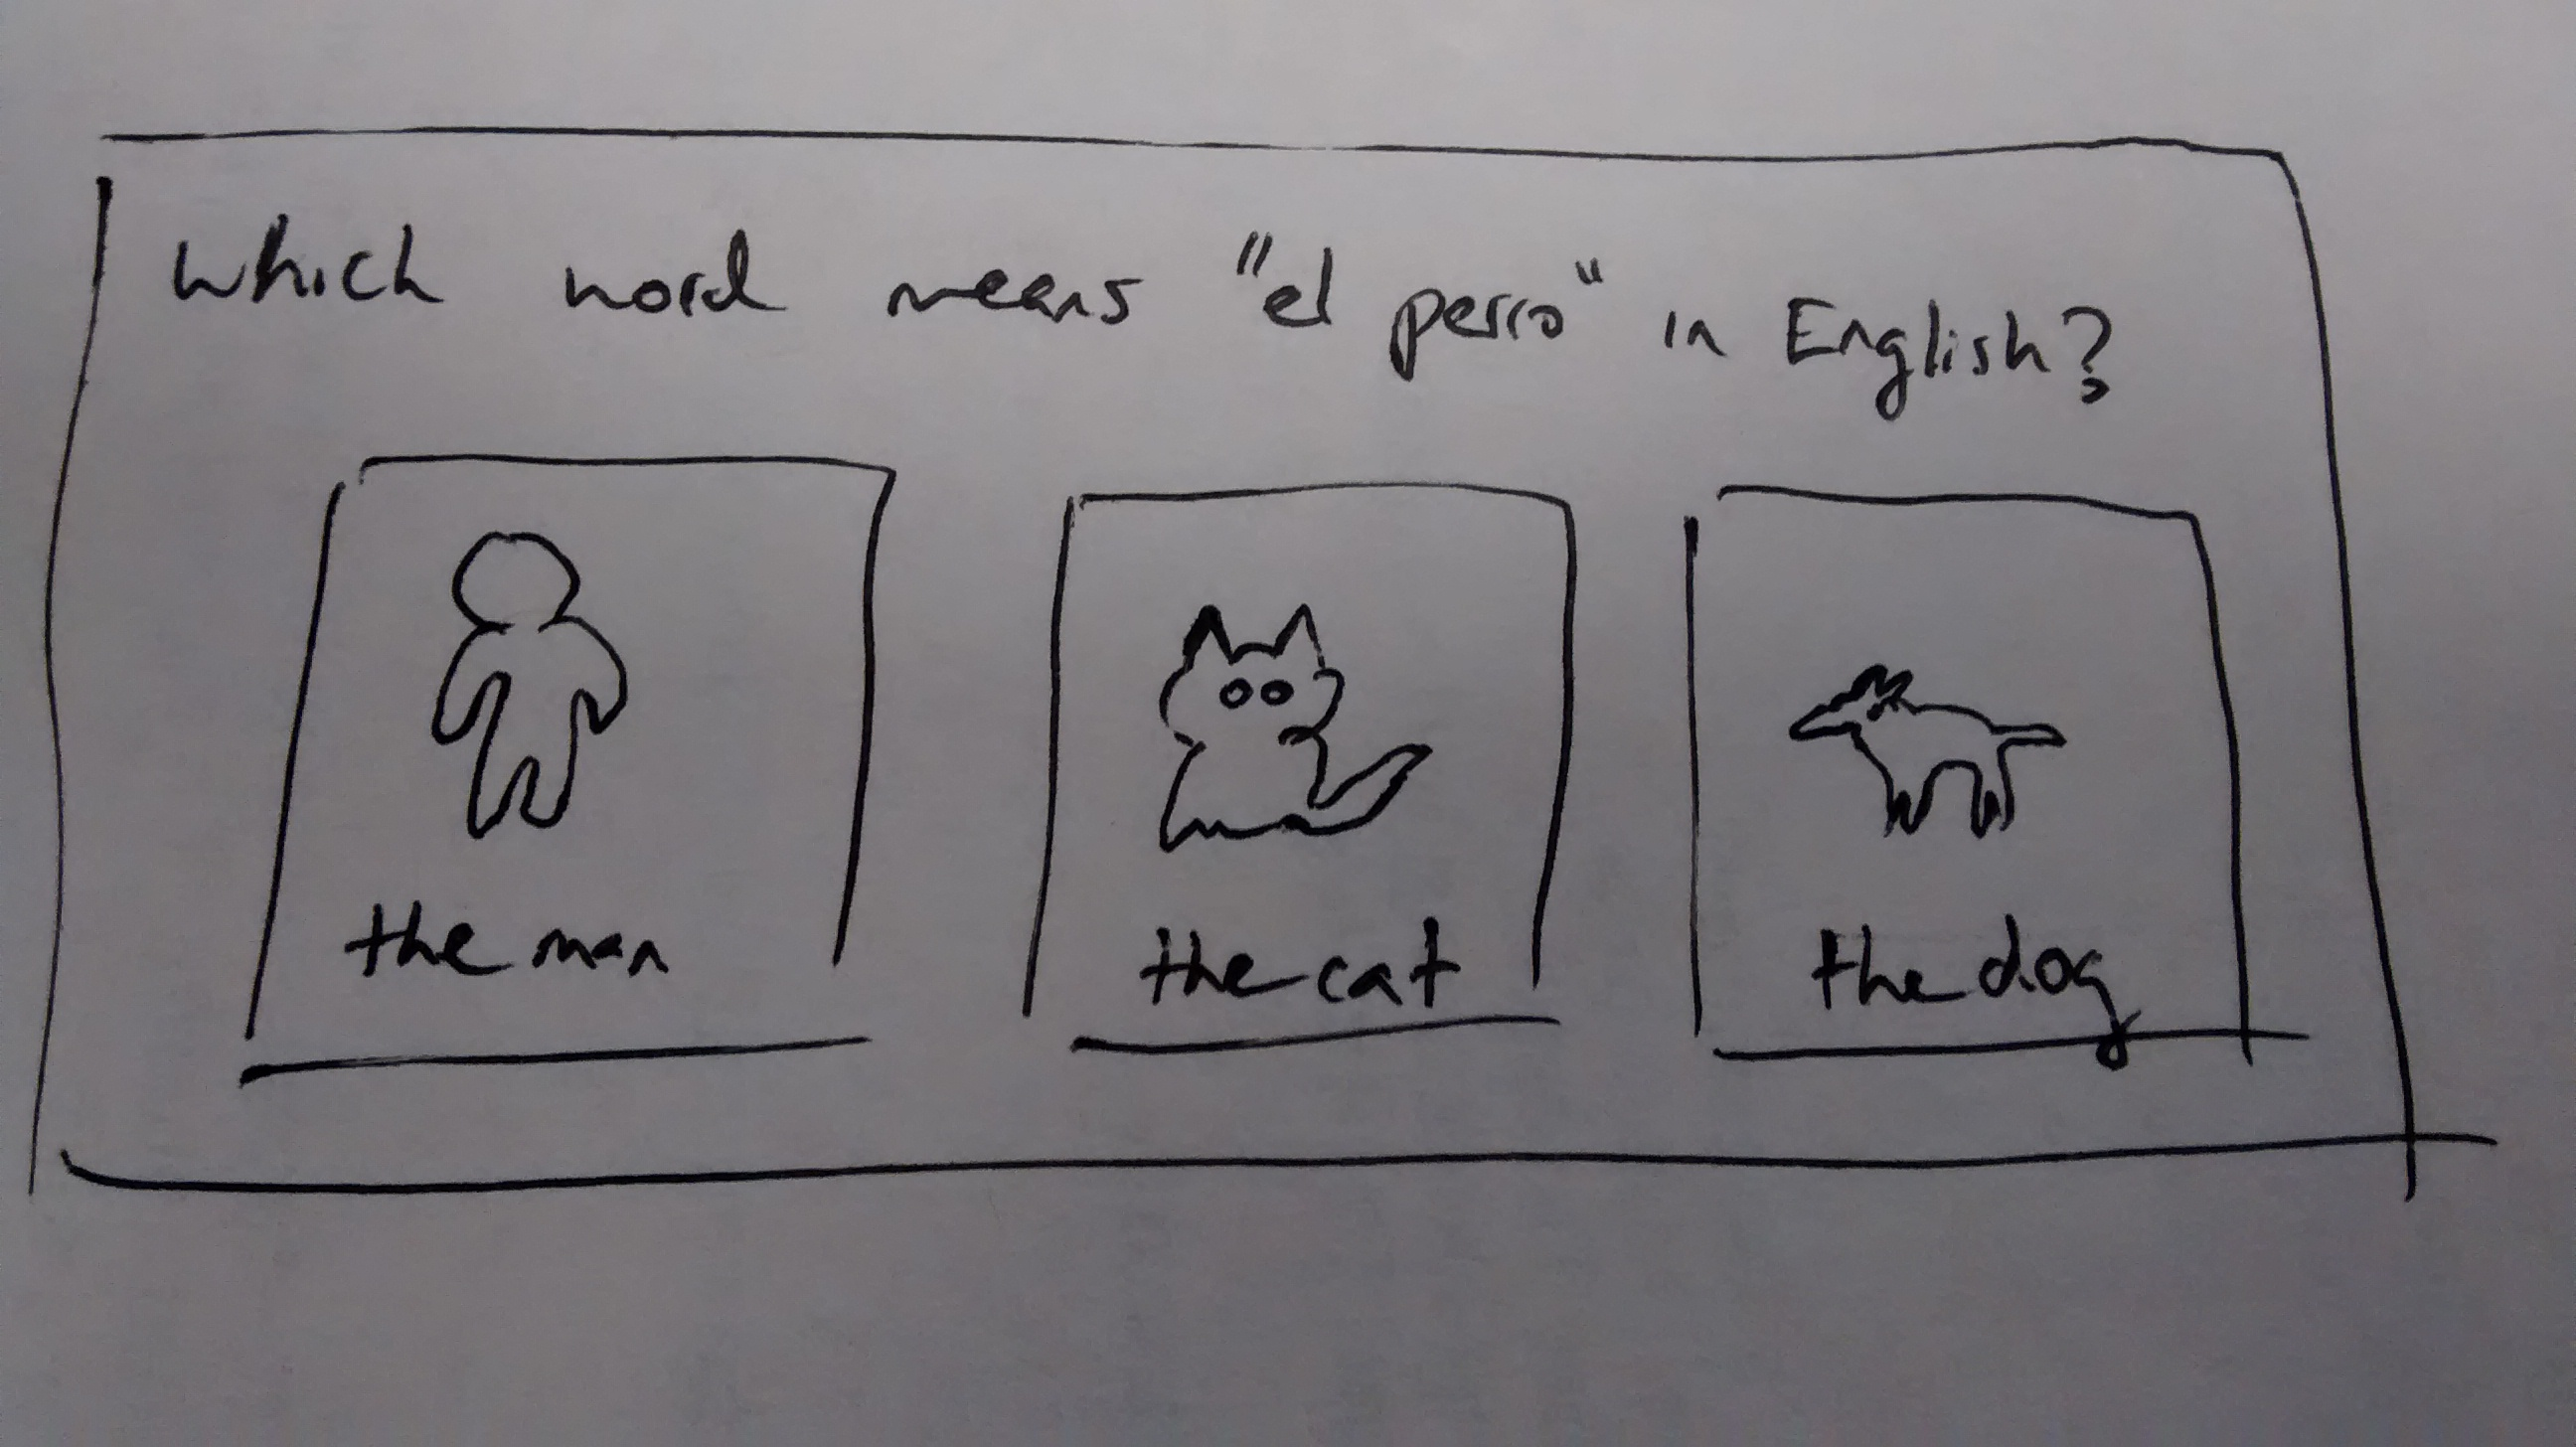
\includegraphics[width=1.0\columnwidth]{quiz2}
%\caption{Another type of quiz presents a noun in English (umbrella), and asks the user to select the correct translation into Japanese (\textit{kasa}). The user has incorrectly selected \textit{fukuro}, so the user is shown its meaning (bag), and tries again.}
\caption{One type of quiz presents a noun in English (umbrella), and asks the user to select the correct translation into Japanese (\textit{kasa}). The user has incorrectly selected \textit{fukuro}, so the user is shown its meaning (bag), and tries again.}
\label{fig:quiz2}
\end{figure}

\begin{figure}
\centering
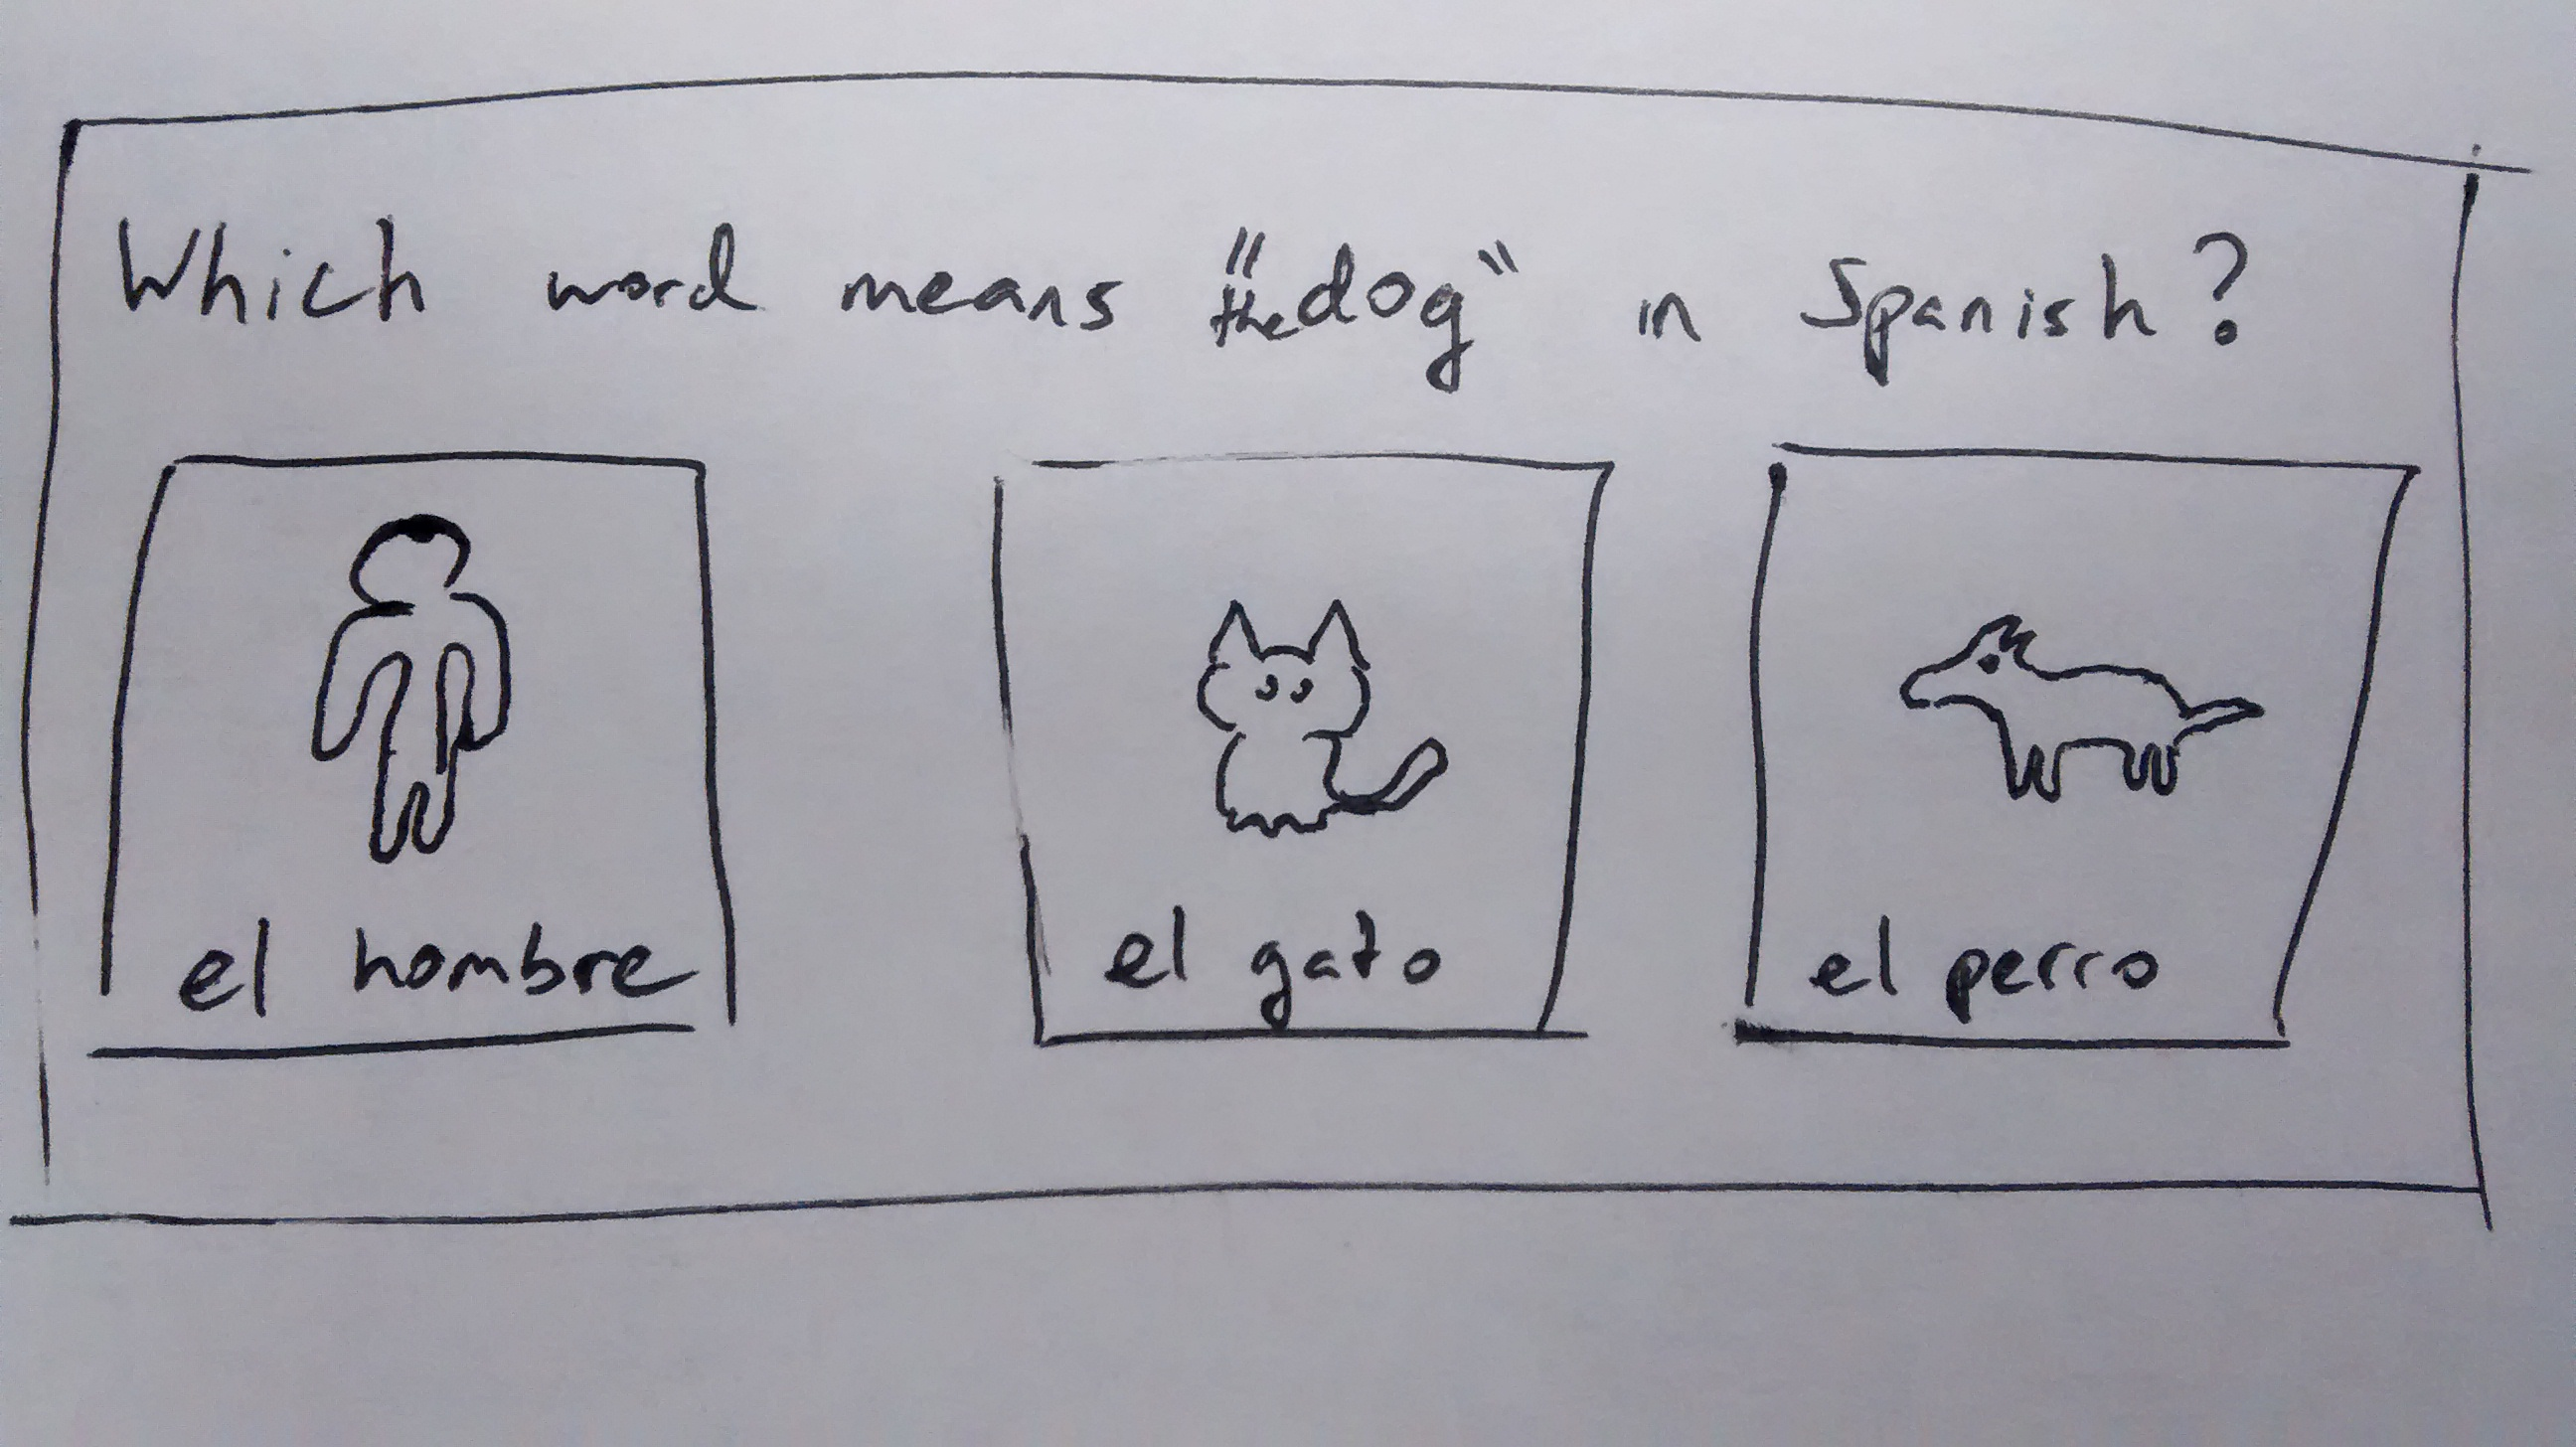
\includegraphics[width=1.0\columnwidth]{quiz1}
\caption{Another type of quiz presents a noun in Japanese (\textit{jikan}), and asks the user to select its meaning (time).}
\label{fig:quiz1}
\end{figure}

We chose this multiple-choice quiz format, because it tests the user's knowledge with a minimal amount of interaction -- the user simply clicks on a word to answer. Once the user answers a quiz correctly, a new quiz testing a different word is displayed. Thus, users can engage with an Edvertisement to continue study vocabulary for as long as they wish to.

% A picture is also presented alongside the foreign-language word, to help learners visually remember them. Prior research has shown that flashcards showing a picture along with the text allow learners to learn vocabulary better than text-only flashcards \cite{multimediavocabulary}. We focus on nouns, because they are the most common type of word -- the majority of words in the Oxford English dictionary are nouns \cite{microlearning} -- and they are relatively easy to visualize. This is the same quiz style used by Duolingo to introduce nouns.

% We opt to use this interactive quiz format, rather than simply showing pairs of words and translations or asking users to explicitly recall and type out translations for words, because it allows us to take advantage of the testing effect with a minimal amount of interaction -- the user simply clicks on a word to answer. Once the user answers a quiz correctly, a new quiz testing a different word is shown. Thus, users can continue to study in their feed for as long as they wish to.

 \subsection{Quiz Generation}

We obtained words and translations from the Nouns section of Wiktionary's 1000 Basic Japanese Words list. We excluded loanwords that users would easily recognize (\textit{pinku}=pink), and words that become homographs when romanized (\textit{hana}=flower or nose). We focus on nouns, because they are the most common type of word \cite{microlearning}. % -- the majority of words in the Oxford English dictionary are nouns % FeedLearn can optionally show the word in the native script (kana/kanji for Japanese), or display a picture of the word. However, we did not show these in our user study, because our users could not read Japanese scripts, and not all words can be visualized with a picture (ex: year).

\pagebreak

\subsection{Spaced Repetition}

Spaced repetition algorithms schedule items for review to ensure long-term retention \cite{karpicke2011spaced}. We modified the Memreflex algorithm \cite{memreflex} to show the overdue word that appeared least recently in the feed (or to introduce a new word if there are no overdue words), instead of always showing the most overdue word. % as Memreflex does.
This ensures that users will continue to see different words as they are scrolling through their feeds, even if they are not always answering the in-feed quizzes.

% Spaced repetition algorithms schedule items for review to ensure long-term retention \cite{spacedrepetition}. We modified the Memreflex algorithm \cite{memreflex} to show the word due for review that has been seen least recently in the feed, as opposed to always showing the most overdue word as Memreflex does. This ensures that users will continue to see different words as they are scrolling through their feeds, even if they are not always answering the in-feed questions.

% Quizzes are generated automatically from the provided English word. The other options are generated by looking up the word in WordNet \cite{wordnet}, to find related words that have similar category and semantics but have different meaning (for example, other animal names). The images are obtained by taking the first result on Google Images. We select the list of words to teach based on their overall usefulness in the language (as judged by word frequency in natural-language text).

%\subsection{Inserting Quizzes into Feeds}

%We insert quizzes into feeds so that they will be encountered at a rate of 1 quiz every 10 posts. We picked this rate, as this was similar to the frequency we observed advertisements and sponsored content appearing in Facebook news feeds. Hence, our should not distract users any more than existing advertisements. %on Facebook. % This is optimal because (need justification).

\section{User Study}

We conducted a preliminary user study to see how frequently users would engage with Edvertisements, and compare the effectiveness of embedded interactive quizzes that can be done without leaving the page, versus inserting static links as is done by today's advertisements and sponsored Facebook posts. %compare the effectiveness of inserting interactive quizzes directly into users' Facebook feeds, versus inserting links to the quizzes as is commonly done on Facebook today. % We compared the 

% have a figure illustrating that usage did not decrease over itme

In our study, we only inserted Edvertisements into Facebook feeds, and did not manipulate advertisements, since many users were already using ad-blockers. Furthermore, manipulating the Facebook feed enabled us to better control the frequency and size of inserted quizzes, compared to repurposing advertisement slots. %, size, and appearance of quizzes. % compared to the limited flexibility afforded by repurposing advertisement slots.

% In our study, we only inserted microlearning tasks into Facebook feeds and did not replace ads with quizzes, as Facebook feeds were an environment we could better control the frequency with which quizzes appeared, their size and appearance, and many interested users were already using ad-blockers, which would have conflicted with the ad-replacement functionality.

\subsection{Participants}

We recruited 12 users (5 female, 7 male) who had not previously studied Japanese but were interested in learning some basic vocabulary. They were voluntary participants recruited from online forums and Facebook groups related to Japanese culture. All of our participants self-reported that they were regular users of Facebook. %, spending at least 10 minutes on the site each day.

% We conducted a 2-week between-subjects user study to evaluate the effectiveness of our system in teaching foreign-language vocabulary.

% We recruited 30 college students with no prior exposure to Japanese, who were interested in learning some basic vocabulary in Japanese. All of our participants were regular users of Facebook, spending at least 10 minutes on the site each day.

\begin{figure}
\centering
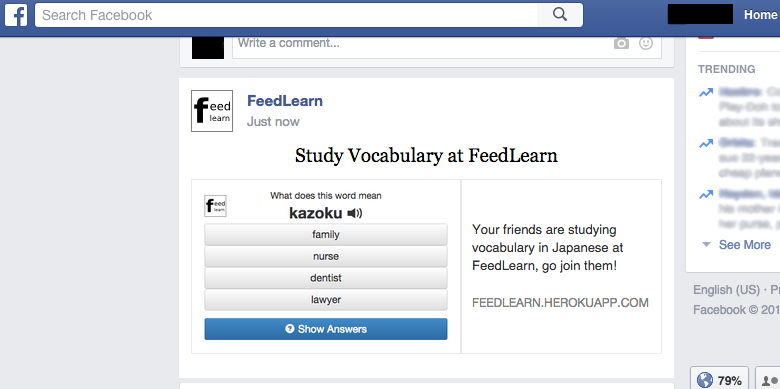
\includegraphics[width=1.0\columnwidth]{feedlearn-link-screenshot}
\caption{The control condition in our user study inserted a link into users' Facebook feeds that led them to a site where they could do quizzes.}
\label{fig:control}
\end{figure}

\subsection{Materials}

We selected 50 basic Japanese words from Wiktionary's Basic Japanese Words list as the study material. We presented vocabulary words in romanized form instead of Japanese script, since our users could not read Japanese script.

%We selected the 30 most frequently used non-abstract nouns in Japanese, and generated flashcards automatically for them, according to the procedure described in the Quiz Generation section. We presented vocabulary words in romanized form rather than the standard Japanese orthography, to avoid difficulties resulting from unfamiliarity with the Japanese writing system.

\subsection{Conditions}

Users were assigned to one of two conditions:

\begin{compactitem}
\item Users in the \textit{in-feed quiz} condition had quizzes inserted directly into their feeds, as shown in \autoref{fig:feedlearn}.
\item Users in the \textit{link} condition were shown links to a site where they could do the quizzes, as shown in \autoref{fig:control}.
\end{compactitem}

Apart from the different items (quizzes/links) inserted into the feed, the questions and quiz interfaces were identical in both conditions. In both conditions, the items were inserted at a rate of 1 quiz/link per 10 feed items. % We chose this rate because it was approximately the rate at which we observed sponsored content and advertisements to appear in our feeds.

% There were 3 conditions in our study. We assigned 10 students to each:

\subsection{Procedure}

The study was conducted entirely online. First, users took a pre-test where they tried matching the 50 Japanese words to their 50 English definitions. Then they installed our Chrome extension and used it to study the 50 words for a week. After a week, we asked users to take the post-test, which had the same format as the pre-test.

% The study was conducted entirely online. First, users took a pre-test on the words we were intending to teach them, where they tried matching the 50 Japanese words to their 50 English definitions. Then they installed our Chrome extension and used it to study the 50 words for a week. After a week, we asked users to do the post-test, which had the same format as the pre-test.

\section{Results}

\subsection{Vocabulary Quiz Results}

\begin{figure}
\centering
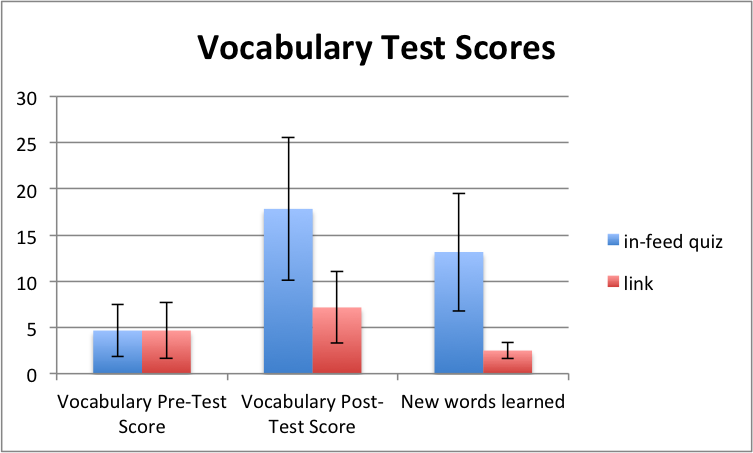
\includegraphics[width=1.0\columnwidth]{vocab-test-scores}
\caption{Vocabulary test scores for the in-feed quiz and link conditions, with standard error bars}
\label{fig:vocab-test-scores}
\end{figure}

\autoref{fig:vocab-test-scores} shows average vocabulary pre-test and post-test scores. On average, users in the in-feed condition learned 13.2 new words, compared to 2.5 new words in the link condition. However, this difference was not statistically significant (t=1.51, p=0.16).

\subsection{Engagement With Edvertisements}

\autoref{fig:event-logs} shows the number of times users practiced answering quizzes. We also kept track of ``study sessions'', which we defined as the number of times the user clicked on the link to visit the website (in the link condition), or first engaged with an Edvertisement (in the in-quiz condition). % We also show number of answers and sessions normalized by the number of feed insertions to normalize for amounts of Facebook use.

\begin{figure}
\centering
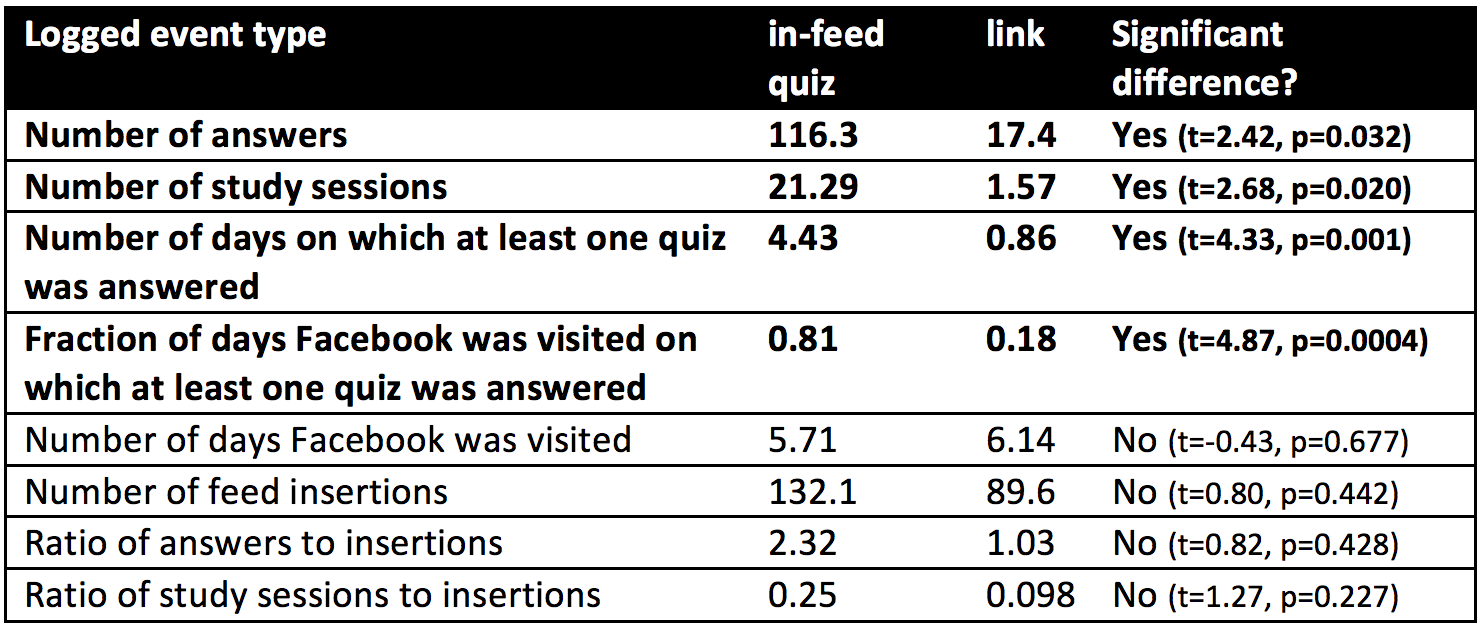
\includegraphics[width=1.0\columnwidth]{event-logs-feedlearn}
\caption{Average number of events logged per user for the in-feed quiz and link conditions.}
\label{fig:event-logs}
\end{figure}

We found that there was high engagement with in-feed Edvertisements -- on average, users answered 116 quizzes across 21 study sessions and answered a question 4.4 days of the 5.7 days they visited Facebook. Users in the in-feed quiz condition answered significantly more quizzes than the link condition, engaged in more study sessions, and studied on more days across the week. % We believe this difference is due to the decreased barrier to starting a study session in the in-feed condition, as they do not need to leave the feed.

\pagebreak

\subsection{Qualitative Feedback}

Some users mentioned that they would prefer words to be explicitly introduced first before they start appearing in quizzes.  In addition, as we can see from the ratio of study sessions to feed insertions, even in the in-feed condition, users only interact with 1/5 of quizzes they see. Hence, we need to ensure that seeing items reinforces memory, even if users do not interact with them. To address this issue, we later added new types of items to introduce new words and review old ones.

\section{Conclusion and Future Work}

Edvertisements are interactive microlearning tasks that we can show to users as they are surfing the web. We have built a browser extension that can show Edvertisements by inserting them into Facebook feeds, or by replacing web advertisements with them.

In our user study, we inserted Edvertisements teaching vocabulary into users' Facebook feeds. We found that users engaged with and learned from Edvertisements, and that engagement rates were higher when the quizzes could be done without leaving their Facebook feeds.

Our current implementation can insert Edvertisements into Facebook feeds, and can replaces web advertisements with them. There are other online contexts where we might show users Edvertisements -- for example, between Youtube videos, chapters of a e-book, or in their email. Although we have focused on microlearning, Edvertisements could also be used to remind people to do other small, beneficial tasks as they are idly surfing the web -- for example, encouraging people to  do a small exercise, or complete an item on their to-do list. % brush their teeth, do a small exercise, or complete an item on their to-do list.

Other directions for future work include making Edvertisements more personalized and contextually relevant, based on the user's browsing history and social networks. For example, if today is your Chinese friend's birthday and your browsing habits indicate that you are learning Chinese, we might show an Edvertisement in your Facebook feed teaching you how to wish him a happy birthday in Chinese. Or if you are reading an anti-vaccination webpage, an Edvertisement might teach you scientific facts about vaccines, showing the names of your friends who have also completed that Edvertisement. Or if many of your friends run, we might show you an Edvertisement about the health benefits of running, showing your friends' recent runs as part of the Edvertisement. % Or if you are reading an anti-vaccination webpage, an Edvertisement might teach you scientific facts about vaccines.

Production of Edvertisements and monetization is another area of future work. One potential approach is sponsored Edvertisements -- for example, a local gym might sponsor an Edvertisement which teaches you a workout routine, hoping it'll encourage you to visit their gym.

% related work: budgeting time spent online

People spend hours surfing the web, but many fail to invest time towards learning and other forms of self-improvement. By putting interactive microlearning tasks right in peoples' social feeds and websites, we aim to help users learn in their spare time, one Edvertisement at a time. % we aim to reduce the barrier to learning, one Edvertisement at a time. %Edvertisements hope to reduce the barrier to investing time towards self-improvement. % people towards positive behavior change.

% As evidenced by the rise in ad-blocking, users are growing frustrated at distracting, irrelevant advertisements on webpages and in their social feeds. Edvertisements aims to address this issue, by re-claiming the spaces for purposes like microlearning that will benefit the end user.

% Users are growing frustrated at distracting, irrelevant advertisements on webpages and in their social feeds. Edvertisements aims to help address this issue, by re-claiming the spaces for purposes that will benefit the end user. %, such as microlearning.

% One question that remains is who will produce the de

% We also envision that social learning features could be introduced to Edvertisements. For example, users might be placed into groups around topics of common interest, and send Edvertisements they liked to their friends.

% TODO Discuss potential social aspects of Edvertisements. Might people send them to their friends?

% Like the problem posed by ad-blockers today, an issue with replacing web advertisements with Edvertisements is that websites will be unable to monetize their content. Monetization is another area of future work. One potential approach would be sponsored Edvertisements -- for example, a local gym might sponsor an Edvertisement which teaches you a workout routine, hoping it'll encourage you to visit their gym. % Alternatively, one might investigate effects of having a mix of Edvertisements and normal ads. It would be interesting if, for example, the presence of Edvertisements starts making people pay more attention to web advertising in general.

% We have presented 

% Just like the problem posed by ad-blockers today, an issue with entirely replacing web advertisements with Edvertisements is that websites will be unable to monetize their content. Making this system acceptable and appealing to advertisers is another area of future work. One potential approach would be sponsored Edvertisements -- for example, a local gym might sponsor an Edvertisement which teaches you an workout routine, hoping it'll encourage you to visit their gym more. Alternatively, one might investigate effects of replacing only some of the ads, and having a mix of Edvertisements and traditional advertisements. It would be interesting if, for example, the presence of Edvertisements starts making people pay more attention to web advertising in general.

\section{Edvertisements Demo and Source Code}

Researchers interested in using or building on Edvertisements can visit \url{https://edvertisements.github.io/}

\pagebreak

% FeedLearn uses Facebook feeds for vocabulary microlearning.
% By eliminating the need to leave the Facebook feed to do quizzes, FeedLearn reduces the barrier
% required to start microlearning tasks. Our user study found that eliminating the need to click a link to start studying vocabulary results in increased engagement.

% We have thus far focused on interactive microlearning tasks in -- Facebook feeds, and replacing web advertisements. There are many other contexts where we might show users relevant microlearning tasks -- for example, between youtube videos.

% One potentially interesting 

% Future work includes making the microlearning tasks contextually relevant -- for example, if the user is reading articles about 



% Although we have focused on microlearning vocabulary, other content could also be conveyed in the context of social feeds and advertisements.  In-feed messages encouraging small, actionable tasks could also be used to promote habits such as microexercise.

% Future work includes using a model to determine the optimal times to insert microlearning tasks into feeds. Another potential extension is making the microlearning tasks more integrated with the Facebook environment to create a more social in-feed learning experience. %Future work includes better integrating the microlearning tasks with the the social nature of the Facebook environment to create a richer in-feed learning experience.

%\section{Acknowledgements}

%Thanks to James Landay, Michael Bernstein, and the Stanford HCI group for suggestions on this project. Geza Kovacs is supported by the NDSEG fellowship.

%Although we have focused on vocabulary learning, this approach can potentially be applied to other educational content, or even be used to encourage other small, actionable behaviors such as microexercise. % One could also use a similar mechanism to encourage other behaviors that need to be done for short periods of time on a daily basis, such as small amounts of exercise.

%Potential future work includes using an adaptive model to determine the optimal times to insert microlearning tasks into feeds. Another potential extension of this work is making the microlearning tasks more integrated with the Facebook environment to create a more social in-feed learning experience.

% The study is conducted entirely online. First, we ask the users to take a pre-test, to verify that they do not already know the vocabulary that we intend to teach them. The test is a multiple choice test: there are 30 questions total, with 15 questions where questions where the user is given the foreign-language word and is asked to select the correct English translation, and 15 questions where the user is given a word in English and is asked to select the correct foreign translation.

% Then, we have them install our extension have them use the service for 2 weeks (according to the condition they have been assigned to). After the 2 weeks have elapsed, we again ask them to take the vocabulary quiz.

%\subsection{Research Questions}

%H1: Do users learn more vocabulary in the FeedLearn condition than the other conditions?

%H2: Do user engage more (complete more quizzes) in the FeedLearn condition than the other conditions?

%H3: Do users enjoy the FeedLearn condition more than the other conditions?

%\section{Results}

%H1: Hopefully, we find that the amount of vocabulary learned in the FeedLearn condition is greater than the other two conditions

%H2: Hopefully, we find the users engage more (complete more quizzes) in the FeedLearn condition than the other conditions.

%H3: Hopefully, we find that users find injection of quizzes directly into their Facebook feeds less distracting than injection of reminders for them to visit the site, or email-based reminders.

% \section{Discussion}

% Although in all 3 conditions, users receive daily reminders to go study vocabulary, we found that users complete more quizzes in the FeedLearn condition, and consequently learn more vocabulary.

% Relative to the External Service with In-Feed Reminders condition, we can attribute this to the reduced friction required for the interaction: the user no longer needs to leave their news feed and visit an external service to review vocabulary, so the barrier to engagement is lowered by inserting vocabulary quizzes directly into social feeds.

% Relative to the External Service with Email Reminders condition, we can additionally attribute an advantage to being able to catch them when they are idle and free. While the user may be busy at 10AM and not have time when they receive the email to review the vocabulary, and will consequently have to remember to go visit the site at a later time, users in the FeedLearn condition have already indicated that they are free and idle because they are browsing their news feed, and are hence more likely to be available to review vocabulary when they encounter them in their feeds.

% Users found the FeedLearn condition more enjoyable and less distracting than the External Service with Email Remdiners condition, because they were able to directly go engage with the quiz content, and were not distracted by unnecessary reminder emails.

\balance{}

% REFERENCES FORMAT
% References must be the same font size as other body text.
\bibliographystyle{SIGCHI-Reference-Format}
\bibliography{edvertisements}

\end{document}

%%% Local Variables:
%%% mode: latex
%%% TeX-master: t
%%% End:

